\documentclass[12pt,a4paper,bibliography=totocnumbered,listof=totocnumbered]{scrartcl}
%\usepackage[german]{babel}
%\usepackage{german}
\usepackage[ngerman]{babel} 
\usepackage[utf8]{inputenc}
%\usepackage[T1]{fontenc} 
\usepackage{amsmath}
\usepackage{amsfonts}
\usepackage{amssymb}
\usepackage{graphicx}
\usepackage{fancyhdr}
\usepackage{tabularx}
\usepackage{geometry}
\usepackage{setspace}
\usepackage[right]{eurosym}
\usepackage[printonlyused]{acronym}
\usepackage{subfig}
\usepackage{floatflt}
\usepackage{float}
\usepackage[usenames,dvipsnames]{color}
\usepackage{colortbl}
\usepackage{paralist}
\usepackage{array}
\usepackage{titlesec}
\usepackage{parskip}
\usepackage[right]{eurosym}
%\usepackage{picins}
\usepackage[subfigure,titles]{tocloft}
\usepackage[hidelinks]{hyperref}
\usepackage{epstopdf}
\epstopdfsetup{update} % only regenerate pdf files when eps file is newer
\usepackage{url}
\usepackage{svg}
\usepackage[toc,page]{appendix}
\usepackage{tikz}
\usetikzlibrary{decorations.pathreplacing}


% Kaputte Zeilenumbrueche fixen
\setlength{\emergencystretch}{1em}

%%% PATH SETTINGS %%% 
\graphicspath{ {pics/} }

\usepackage{listings}
\lstset{basicstyle=\footnotesize, captionpos=b, breaklines=true, showstringspaces=false, tabsize=2, frame=lines, numbers=left, numberstyle=\tiny, xleftmargin=2em, framexleftmargin=2em}
\makeatletter
\def\l@lstlisting#1#2{\@dottedtocline{1}{0em}{1em}{\hspace{1,5em} Lst. #1}{#2}}
\makeatother

\geometry{a4paper, top=27mm, left=30mm, right=20mm, bottom=35mm, headsep=10mm, footskip=12mm}

\begin{document}

\titlespacing{\section}{0pt}{12pt plus 4pt minus 2pt}{-6pt plus 2pt minus 2pt}

% Kopf- und Fusszeile
\renewcommand{\sectionmark}[1]{\markright{#1}}
\renewcommand{\leftmark}{\rightmark}
\pagestyle{fancy}
\lhead{}
\chead{}
\rhead{\thesection\space\contentsname}
%\lfoot{TODO: Short Title}
\cfoot{}
\rfoot{\ \linebreak Page \thepage}
\renewcommand{\headrulewidth}{0.4pt}
\renewcommand{\footrulewidth}{0.4pt}

% Vorspann
\renewcommand{\thesection}{\Roman{section}}
\renewcommand{\theHsection}{\Roman{section}}
\pagenumbering{Roman}

% ----------------------------------------------------------------------------------------------------------
% Titelseite
% ----------------------------------------------------------------------------------------------------------
\thispagestyle{empty}
\begin{center}
	%
\includegraphics[scale=1,natwidth=1691, natheight=458]{logo.jpg}\\
	\vspace*{2cm}
	
	\textbf{codeFEST 8}\\
	\vspace*{2cm}
	\Huge
	\textbf{Projekt \glqq Aix Cruise\grqq}\\
	\vspace*{0.5cm}
	\large
	\vspace*{1cm}
	\Large
	\textbf{Prototyp zur Gamification des Fahrerlebnisses \glqq Aix Cruise\grqq}\\
	\vspace*{2cm}
	
	\vfill
	\normalsize
	\newcolumntype{x}[1]{>{\raggedleft\arraybackslash\hspace{0pt}}p{#1}}
	\begin{tabular}{x{6cm}p{7.5cm}}
		\rule{0mm}{5ex}\textbf{von:} & Alexander Devaykin \newline alexander.devaykin@rwth-aachen.de \\
		\rule{0mm}{5ex}  & Torsten Kohn \newline hello@torstenkohn.de  \\
		\rule{0mm}{5ex}  & Lukas Körfer \newline lukas.koerfer@rwth-aachen.de  \\
		\rule{0mm}{5ex}  & Kevin Leonardic \newline kevin.leonardic@rwth-aachen.de  \\
		
		\rule{0mm}{5ex}\textbf{Datum:} & \today \\ 
	\end{tabular} 
\end{center}
\pagebreak

% ----------------------------------------------------------------------------------------------------------
% Abstract
% ----------------------------------------------------------------------------------------------------------
\setcounter{page}{1}
\onehalfspacing
\titlespacing{\section}{0pt}{12pt plus 4pt minus 2pt}{2pt plus 2pt minus 2pt}

\rhead{Einführung}

%Das Dokument muss immer doppelt kompiliert werden, weil nach dem ersten Mal die meisten Änderungen noch nicht in der PDF-Datei zu sehen sind.
\section{Einführung}
Dieses Dokument soll grob die Funktionalität des Prototypen \glqq Aix Cruise\grqq welcher im Rahmen des codeFEST8 entstanden ist umreißen. Das Ziel hierbei ist eine Übersicht über bereits implementierte Features zu gewinnen sowie mögliche Ausblicke zu gewähren. Hierbei wird sowohl auf die verwendete Technologie, als auch die zugrundeliegenden Gedankengänge eingegangen.
Bei \glqq Aix Cruise\grqq handelt es sich um ein Projekt welches auf spielerische Weise ( Stichwort "Gamification" ) das Fahrverhalten des Anwenders analysiert um ihm einen Anreiz zu geben dieses zu Verbessern. 
Dabei soll es möglich sein sich mit Freunden zu vergleichen und seine Erfolge zu Teilen. Kern dieser Idee ist, dass der soziale Druck für akzeptables Fahrverhalten eine besserung desselben zur Folge hat.

\rhead{Die App}
\section{Ist-Zustand}
Das Projekt besteht aus 3 wesentlichen Komponenten.
Die Android App ( "Frontend" ), programmiert in Java mit nativen Funktionen
Die Serversoftware ( "Backend" ), programmiert in Java
Die Datenbank, basierend auf PostgreSQL.

Das Frontend präsentiert die Daten welche durch eine REST-Schnittstelle vom Server bezogen werden auf eine leicht verständliche Weise.
Die genannten Daten umfassen eine Visualisierung der zurückgelegten zusammenhängenden Streckenabschnitte ( Im folgenden "Trip" genannt ) sowie eine kleine Übersicht über relevante Fahrdaten. Momentan umfasst dies die zurückgelegte Distanz und den absoluten Spritverbrauch der kompletten Strecke.

Das Backend exponiert die in der Datenbank gespeicherten Daten über eine RESTful API und bietet die Möglichkeit einer Authentifizierung. Diese wird allerdings momentan nicht genutzt.

Die Datenbank verwendet PostgreSQL mit dem Funktionserweiterndem Paket postgis, welches es auf einfache Weise ermöglicht geospatiale Auswertungen auf Queryebene auszuführen. Dies reduziet den Aufwand auf der Backendseite erheblich. Mit Hilfe von "Materialized Views" ist es möglich auch komplexe Auswertungen auf effiziente Weise zu Berechnen und zu Speichern. Diese Möglichkeit wird aktuell leider noch nicht genutzt.

\section{Begründung der Wahl der Komponenten}
Die Wahl fiel auf die genannten Softwarepakete, da im Entwicklerteam Erfahrung mit den Systemen vorlag. Es ermöglichte uns eine weitestgehend unabhängige Entwicklung was den Aufwand verringerte, und die Entwicklungsgeschwindigkeit erheblich erhöhte. 
Für Android existiert eine effiziente und frei verfügbare Entwicklungsumgebung, welche auch den damit unerfahrenen Entwicklern einen schnellen Einstieg ermöglichte.
Das Backend ist Teil der Bachelorarbeit von Torsten. Dementsprechend schnell konnte er damit einen Prototypen anfertigen.
Die Datenbank mit Plugin wurde von Kevin bereits in der Vergangenheit erfolgreich in ähnlicher Weise genutzt.

\section{Funktionalität die nicht vorhanden ist}
Das Aufzeichnen der Fahrt direkt von der OBD-II Schnittstelle ist noch nicht Teil der Anwendung.
Die algorithmische Auswertung der Fahrtdaten ist nicht implementiert. Die "Achievements" wurden manuell erfasst und eingetragen.
Jegliche Interaktion des Frontends mit dem Backend bei welcher das Frontend den Server dazu veranlassen müsste Daten zu speichern ist noch nicht implementiert. Dies wäre z.B. beim Hinzufügen von Freunden der Fall.

\section{Aussicht}

Es ist denkbar die Software zu Erweitern (beziehungsweise komplett abzuändern) um den Anforderungen in einem wesentlich größerem Maßstab als dem Hackathon gerecht zu werden.
Zum Beispiel Flottenfunktionalität, die Abschottung einzelner Bereiche, die Gruppierung nach Fahrzeugtyp und Modell und vieles weitere.
Die große Chance von diesem Ansatz ist es, auf einfache Weise viele wertvolle Daten zu gewinnen welche via Data Mining Algorithmen analysiert und gewinnbringend genutzt werden können.
Dabei können bestehende Strategien evaluiert werden und/oder neue Strategien und Erkenntnisse gewonnen werden.

\section{Offensichtliche Limitation des aktuell genutzten Konzepts}

Momenten besteht die einzige Möglichkeit Daten zu Sammeln in der Nutzung von Android in Kombination mit einem OBD-II Dongle. Diese Konstellation ist fehleranfällig und wartungsintensiv.
Das Backend basiert auf selbst entwickelter Software welche nur für den Einsatz im kleinen Umfeld vorgesehen ist. Hier muss ein komplett neuer Ansatz her.
Die Datenbank skaliert möglicherweise ab einem Punkt nicht mehr optimal. Dies müsste sorgfältig evaluiert werden um zukünftige Engpässe zu Vermeiden.

\section{Impressionen}

\begin{table}
\begin{tabular}{c c}

\begin{minipage}{.5\textwidth}
  \centering
  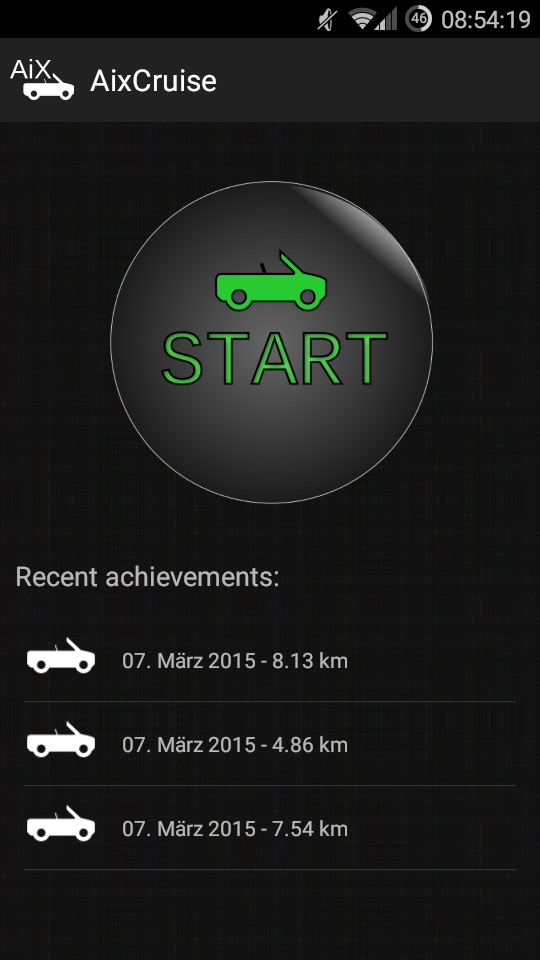
\includegraphics[scale=0.3]{images/main.png}
  \caption{Start Bildschirm}
  \label{main}
\end{minipage}
&
\begin{minipage}{.5\textwidth}
  \centering
  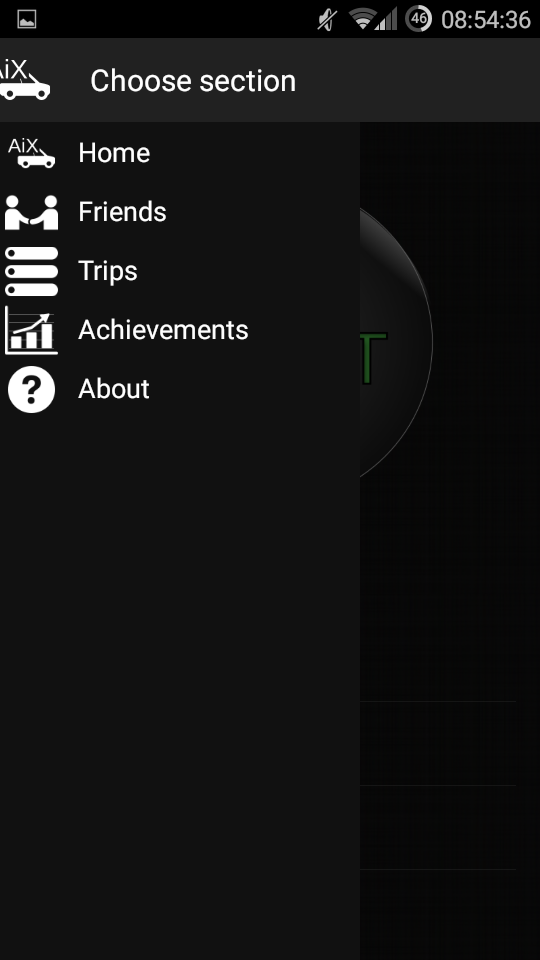
\includegraphics[scale=0.3]{images/menu.png}
  \caption{Menü}
  \label{menu}
\end{minipage}

\end{tabular}
\end{table}
\begin{table}
\begin{tabular}{c c}

\begin{minipage}{.5\textwidth}
  \centering
  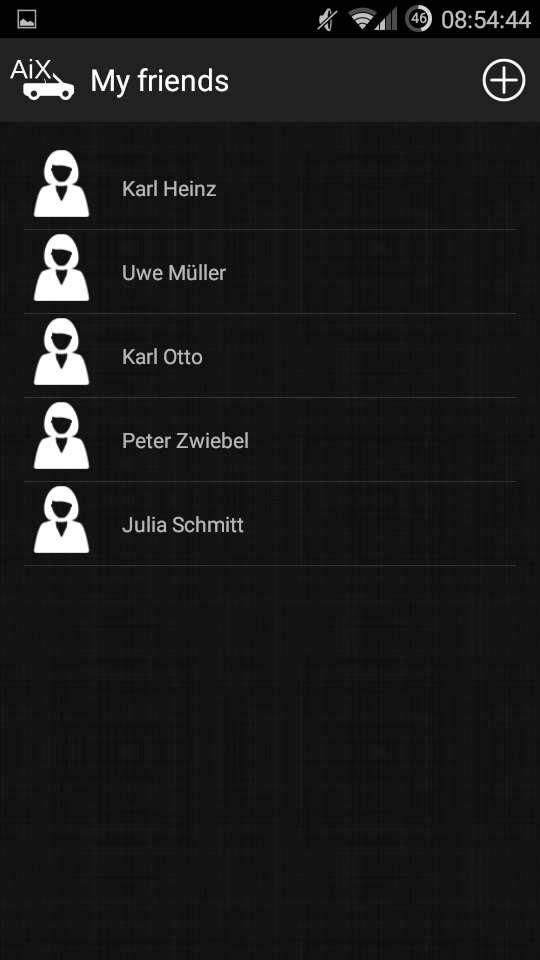
\includegraphics[scale=0.3]{images/friends.png}
  \caption{Freunde}
  \label{friends}
\end{minipage}
\pagebreak
&
\begin{minipage}{.5\textwidth}
  \centering
  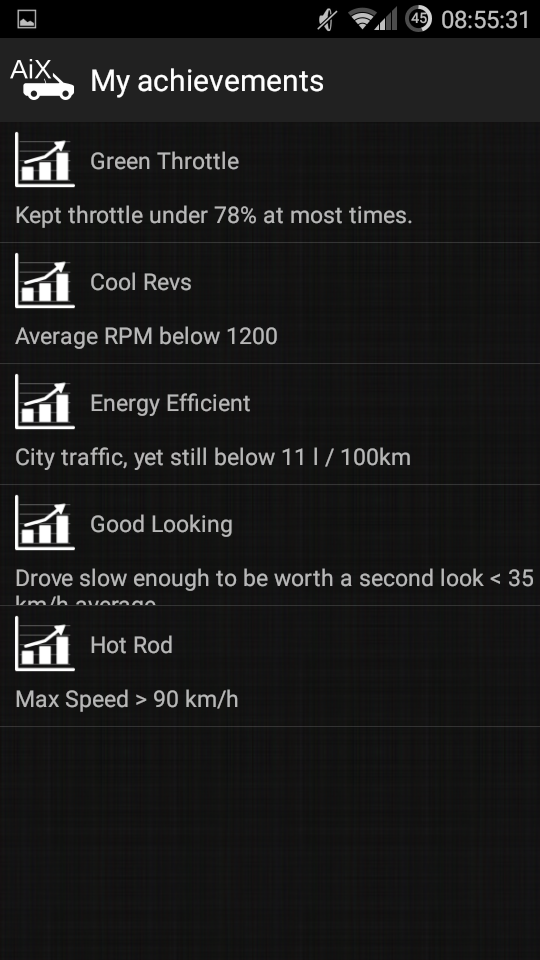
\includegraphics[scale=0.3]{images/achievements.png}
  \caption{\glqq Errungenschaften\grqq}
  \label{achievements}
\end{minipage}

\end{tabular}
\end{table}
\begin{table}
\begin{tabular}{c c}
\begin{minipage}{.5\textwidth}
  \centering
  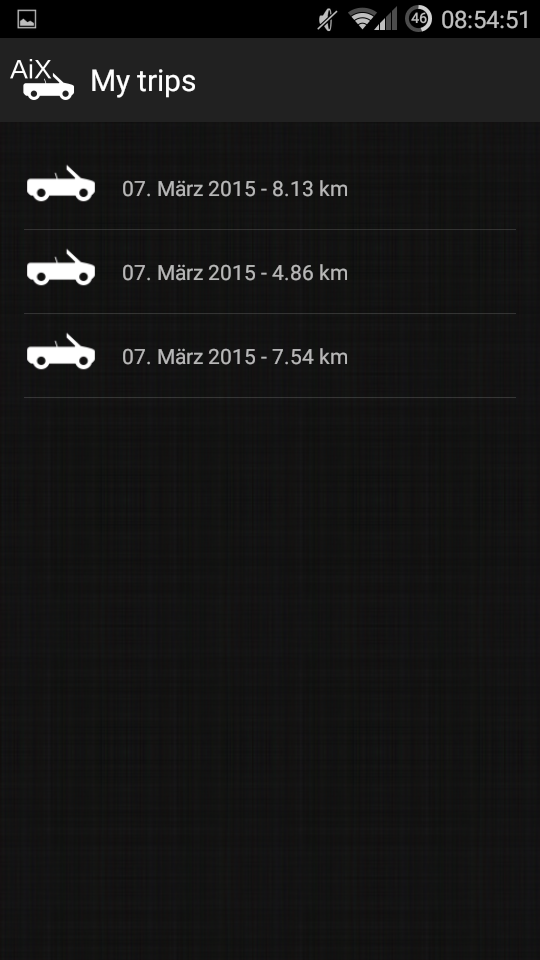
\includegraphics[scale=0.3]{images/trips.png}
  \caption{Fahrtenübersicht}
  \label{trips}
\end{minipage}
&
\begin{minipage}{.5\textwidth}
  \centering
  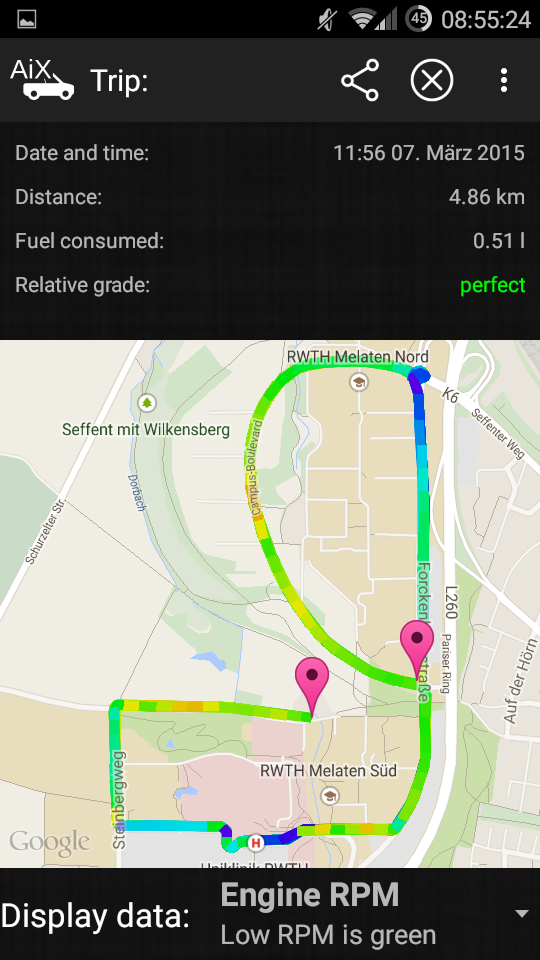
\includegraphics[scale=0.3]{images/trip_detail.png}
  \caption{Detailansicht Fahrt}
  \label{main}
\end{minipage}
\end{tabular}
\end{table}

% Abstände Überschrift
\titlespacing{\section}{0pt}{12pt plus 4pt minus 2pt}{-6pt plus 2pt minus 2pt}
\titlespacing{\subsection}{0pt}{12pt plus 4pt minus 2pt}{-6pt plus 2pt minus 2pt}
\titlespacing{\subsubsection}{0pt}{12pt plus 4pt minus 2pt}{-6pt plus 2pt minus 2pt}

% "Fixes" error
\nocite{*}
% Kopfzeile
\renewcommand{\sectionmark}[1]{\markright{#1}}
\renewcommand{\subsectionmark}[1]{}
\renewcommand{\subsubsectionmark}[1]{}
\rhead{\rightmark}

\onehalfspacing
\renewcommand{\thesection}{\arabic{section}}
\renewcommand{\theHsection}{\arabic{section}}
\setcounter{section}{0}
\pagenumbering{arabic}
%\setcounter{page}{1}

\definecolor{mygreen}{rgb}{0,0.6,0}
\definecolor{mygray}{rgb}{0.5,0.5,0.5}
\definecolor{mymauve}{rgb}{0.58,0,0.82}

\lstset{ %
  backgroundcolor=\color{white},   % choose the background color; you must add \usepackage{color} or \usepackage{xcolor}
  basicstyle=\scriptsize,        % the size of the fonts that are used for the code
  breakatwhitespace=false,         % sets if automatic breaks should only happen at whitespace
  breaklines=true,                 % sets automatic line breaking
  captionpos=b,                    % sets the caption-position to bottom
  commentstyle=\color{mygreen},    % comment style
  deletekeywords={...},            % if you want to delete keywords from the given language
  escapeinside={\%*}{*)},          % if you want to add LaTeX within your code
  extendedchars=true,              % lets you use non-ASCII characters; for 8-bits encodings only, does not work with UTF-8
  frame=single,                    % adds a frame around the code
  keepspaces=true,                 % keeps spaces in text, useful for keeping indentation of code (possibly needs columns=flexible)
  keywordstyle=\color{blue},       % keyword style
  language=Octave,                 % the language of the code
  morekeywords={*,...},            % if you want to add more keywords to the set
  numbers=left,                    % where to put the line-numbers; possible values are (none, left, right)
  numbersep=5pt,                   % how far the line-numbers are from the code
  numberstyle=\tiny\color{mygray}, % the style that is used for the line-numbers
  rulecolor=\color{mygray},         % if not set, the frame-color may be changed on line-breaks within not-black text (e.g. comments (green here))
  showspaces=false,                % show spaces everywhere adding particular underscores; it overrides 'showstringspaces'
  showstringspaces=false,          % underline spaces within strings only
  showtabs=false,                  % show tabs within strings adding particular underscores
  stepnumber=2,                    % the step between two line-numbers. If it's 1, each line will be numbered
  stringstyle=\color{mymauve},     % string literal style
  tabsize=4,                       % sets default tabsize to 2 spaces
  title=\lstname                   % show the filename of files included with \lstinputlisting; also try caption instead of title
}

\end{document}
